%% LyX 2.1.3 created this file.  For more info, see http://www.lyx.org/.
%% Do not edit unless you really know what you are doing.
\documentclass[russian,english]{beamer}
\usepackage[T2A,OT2,T1]{fontenc}
\usepackage[utf8x]{inputenc}
\setcounter{secnumdepth}{3}
\setcounter{tocdepth}{3}
\usepackage{babel}
\usepackage{calc}
\usepackage{amssymb}
\usepackage{graphicx}
\ifx\hypersetup\undefined
  \AtBeginDocument{%
    \hypersetup{unicode=true,
 bookmarks=true,bookmarksnumbered=true,bookmarksopen=false,
 breaklinks=false,pdfborder={0 0 1},backref=false,colorlinks=true,pdftitle={Reviving the Old Russian orthography for the 21st century},
 pdfauthor={Sergei Winitzki},
 pdfsubject={computer word processing},
 linkcolor=black,urlcolor=blue}
  }
\else
  \hypersetup{unicode=true,
 bookmarks=true,bookmarksnumbered=true,bookmarksopen=false,
 breaklinks=false,pdfborder={0 0 1},backref=false,colorlinks=true,pdftitle={Reviving the Old Russian orthography for the 21st century},
 pdfauthor={Sergei Winitzki},
 pdfsubject={computer word processing},
 linkcolor=black,urlcolor=blue}
\fi
\usepackage{breakurl}

\makeatletter

%%%%%%%%%%%%%%%%%%%%%%%%%%%%%% LyX specific LaTeX commands.
\DeclareRobustCommand{\cyrtext}{%
  \fontencoding{T2A}\selectfont\def\encodingdefault{T2A}}
\DeclareRobustCommand{\textcyr}[1]{\leavevmode{\cyrtext #1}}
\AtBeginDocument{\DeclareFontEncoding{T2A}{}{}}


%%%%%%%%%%%%%%%%%%%%%%%%%%%%%% Textclass specific LaTeX commands.
 % this default might be overridden by plain title style
 \newcommand\makebeamertitle{\frame{\maketitle}}%
 % (ERT) argument for the TOC
 \AtBeginDocument{%
   \let\origtableofcontents=\tableofcontents
   \def\tableofcontents{\@ifnextchar[{\origtableofcontents}{\gobbletableofcontents}}
   \def\gobbletableofcontents#1{\origtableofcontents}
 }

%%%%%%%%%%%%%%%%%%%%%%%%%%%%%% User specified LaTeX commands.
\usetheme[secheader]{Boadilla}
\usecolortheme{seahorse}
\title[Old Russian Orthography]{Reviving the Traditional Russian Orthography for the 21st Century}
\author{Sergei Winitzki}
\date{April 24, 2015}
\institute[Versal Group Inc.]{Text By The Bay 2015}

\makeatother

\begin{document}
\frame{\titlepage}
\begin{frame}{Old Russian Orthography: what and why}

\begin{itemize}
\item Classic and modern Russian literature used the ``old'' orthography

\begin{itemize}
\item Pushkin, Turgenev, Dostoyevsky, Tolstoy, Chekhov, Nabokov, ...
\end{itemize}
\item The orthography was reformed in 1918:

\begin{itemize}
\item Replaced \foreignlanguage{russian}{\textbf{\emph{ѣ}}$\rightarrow$е,
\textbf{\emph{ѳ}}$\rightarrow$ф, \textbf{\emph{і}}$\rightarrow$и,
\textbf{\emph{ѵ}}$\rightarrow$и} 
\item 4 letters \foreignlanguage{russian}{\textbf{\emph{Ѣѣ}}, \textbf{\emph{Ѳѳ}},
\textbf{\emph{Іі}}, \textbf{\emph{Ѵѵ}}} were physically removed from
printing presses

\begin{itemize}
\item Often, \foreignlanguage{russian}{\textbf{\emph{Ъъ}}} was also removed
by mistake
\end{itemize}
\item Replaced some prefixes, suffixes, and word endings
\end{itemize}
\item Motivation for reform: ``simplify the spelling''
\item Old orthography continued to be used outside Russia
\end{itemize}
\end{frame}

\begin{frame}{Old Russian orthography: example}


Nabokov, \emph{Storm} (1930)

\includegraphics[width=1\textwidth]{Sirin_-_Groza_1930}
\end{frame}

\begin{frame}{Natural language orthography changes naturally...}


Hobbes, \emph{De cive} (1651)

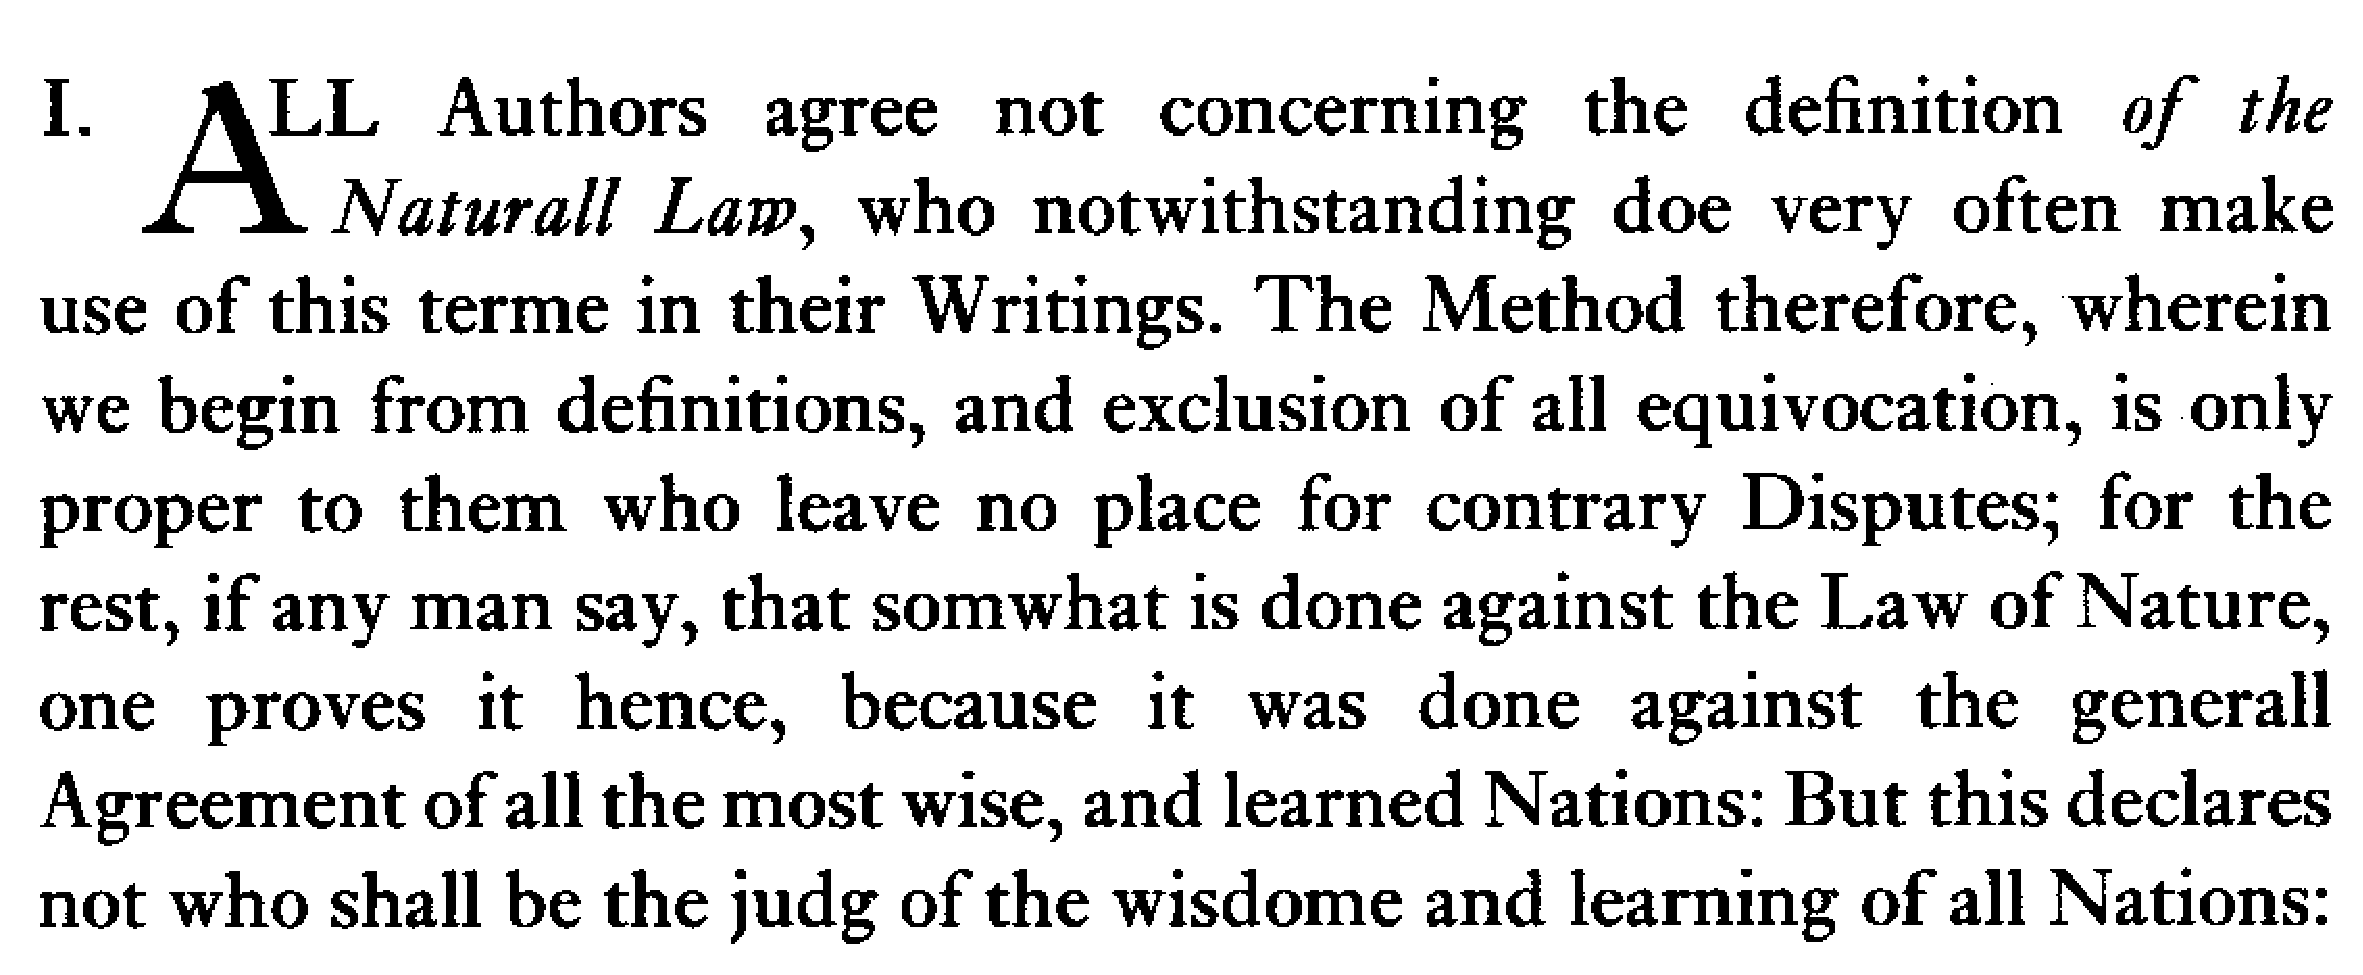
\includegraphics[width=1\textwidth]{Hobbes_-_De_Cive_-_1651}

Some letters are now added: \emph{somwhat}, \emph{judg}

Some letters are now removed: \emph{doe}, \emph{generall}, \emph{wisdome} 
\end{frame}

\begin{frame}{...or when guided by a committee of experts}

\begin{itemize}
\item A proposal for English, similar to the Russian spelling reform...

\begin{itemize}
\item Omit the silent \emph{e} in endings, replace vowels to ``simplify''
spelling

\begin{itemize}
\item breathe $\rightarrow$ breath, some $\rightarrow$ sum, made $\rightarrow$
maid, gate $\rightarrow$ gait
\end{itemize}
\item Replace the letters \emph{c}$\rightarrow$\emph{k}/\emph{s}, \emph{x}$\rightarrow$\emph{ks},
\emph{y}$\rightarrow$\emph{i}

\begin{itemize}
\item played $\rightarrow$ plaid, hence $\rightarrow$ hens, xerox $\rightarrow$
kseroks
\end{itemize}
\item Physically remove the letters \emph{C}, \emph{X}, \emph{Y} from all
computer keyboards

\begin{itemize}
\item because they are a heritage of the \emph{horrible old times} 
\end{itemize}
\end{itemize}
\end{itemize}
\end{frame}

\begin{frame}{What happens if you ban a few letters...}

\begin{itemize}
\item One generation later, nobody remembers anything was ever different
\item You lose effective access to your own culture

\begin{itemize}
\item Cannot print adequate critical editions of classic literature
\item Nobody wants to read even 50-year old books
\item Converting each book to new spelling is hard for editors
\end{itemize}
\item In Russia:

\begin{itemize}
\item People born after $\approx$1950 are loath to read texts in the old
orthography
\item Such texts are perceived to be \emph{unquestionably} obsolete
\item No\emph{ }computers today fully support the old Russian orthography
\end{itemize}
\end{itemize}
\end{frame}

\begin{frame}{Processing old Russian orthography in 2000}


Main challenges:
\begin{itemize}
\item As of 2000, no 8-bit encodings contained the letters \foreignlanguage{russian}{Ѣѣ,
Ѳѳ, Іі, Ѵѵ} 

\begin{itemize}
\item Unicode support was not widespread
\end{itemize}
\item No keyboard layouts, no screen fonts, few vector fonts had them

\begin{itemize}
\item \LaTeX{} font support: nonstandard font encoding made by AMS
\end{itemize}
\item No spelling checker support, no hyphenation, no OCR
\end{itemize}
\end{frame}

\begin{frame}{Back to 2015: State of the art}

\begin{itemize}
\item The letters \foreignlanguage{russian}{Ѣѣ, Ѳѳ, Іі, Ѵѵ} are present
in most (vector) Cyrillic fonts 

\begin{itemize}
\item typesetting, printing supported through Unicode
\item \LaTeX{} font support: OT2 font encoding only!
\end{itemize}
\item Some spelling checker support (\texttt{ispell}, AbiWord, Open Office)
\item Some language support for OCR
\item No hyphenation support, no standard keyboard layouts
\end{itemize}
\end{frame}

\begin{frame}{The \texttt{oldrus-ispell} project (1999-2003)}

\begin{itemize}
\item \href{http://oldrus-ispell.sourceforge.net/koi8-extended.html}{http://oldrus-ispell.sourceforge.net/koi8-extended.html}
\item KOI8-C encoding (\href{http://www.ietf.org/archive/id/draft-winitzki-koi8c-encoding-00.txt}{IETF draft}),
localization for the \href{http://links.twibright.com/}{links} browser
\item A keyboard layout for X-Window and MS Windows 9x
\item Bitmapped X-Window fonts (BDF), the \texttt{xcyr} package

\begin{itemize}
\item Became part of \texttt{\href{http://www.cl.cam.ac.uk/~mgk25/ucs-fonts.html}{ucs-fonts}}
and \texttt{\href{https://packages.debian.org/sid/xfonts-cyrillic}{xfonts-cyrillic}}
\end{itemize}
\item \texttt{ispell} dictionary for old Russian orthography
\item A PostScript typesetter using BDF as Type 3 fonts (Perl)
\item A primitive converter, new $\rightleftarrows$ old orthography (Perl)
\end{itemize}
\end{frame}

\begin{frame}{The KOI8-C encoding and screen fonts}


Viewing Nabokov, \emph{Despair} (1934) in Netscape using KOI8-C

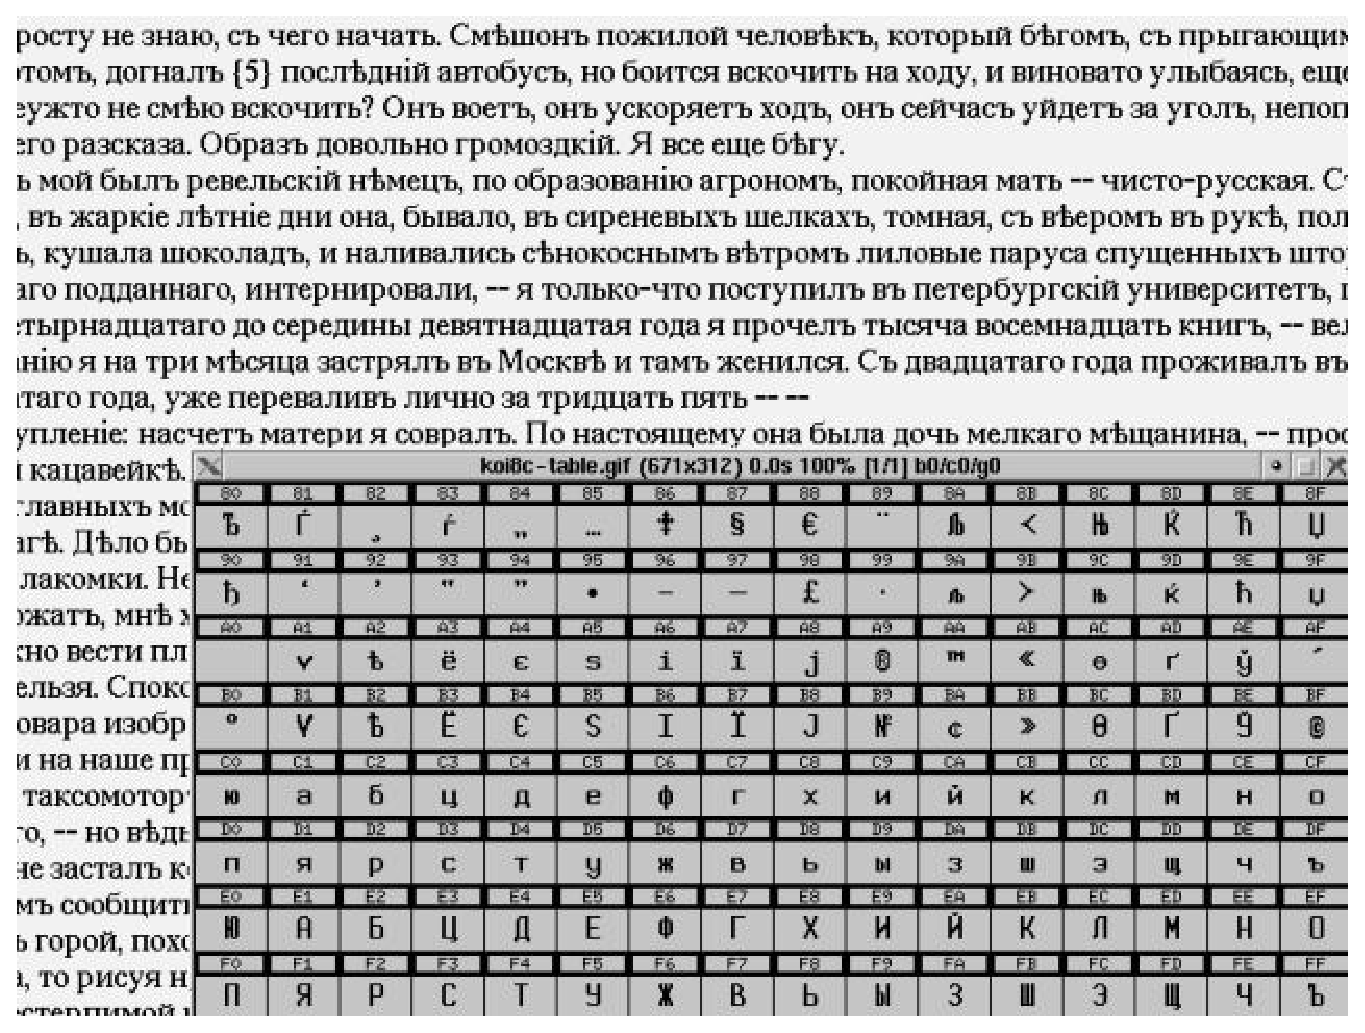
\includegraphics[height=0.8\textheight]{xcyr-screenshot}
\end{frame}

\begin{frame}{Working with the oldrus-ispell dictionary}


Proofreading Melgunov's \emph{Red Terror in Russia} (1924)

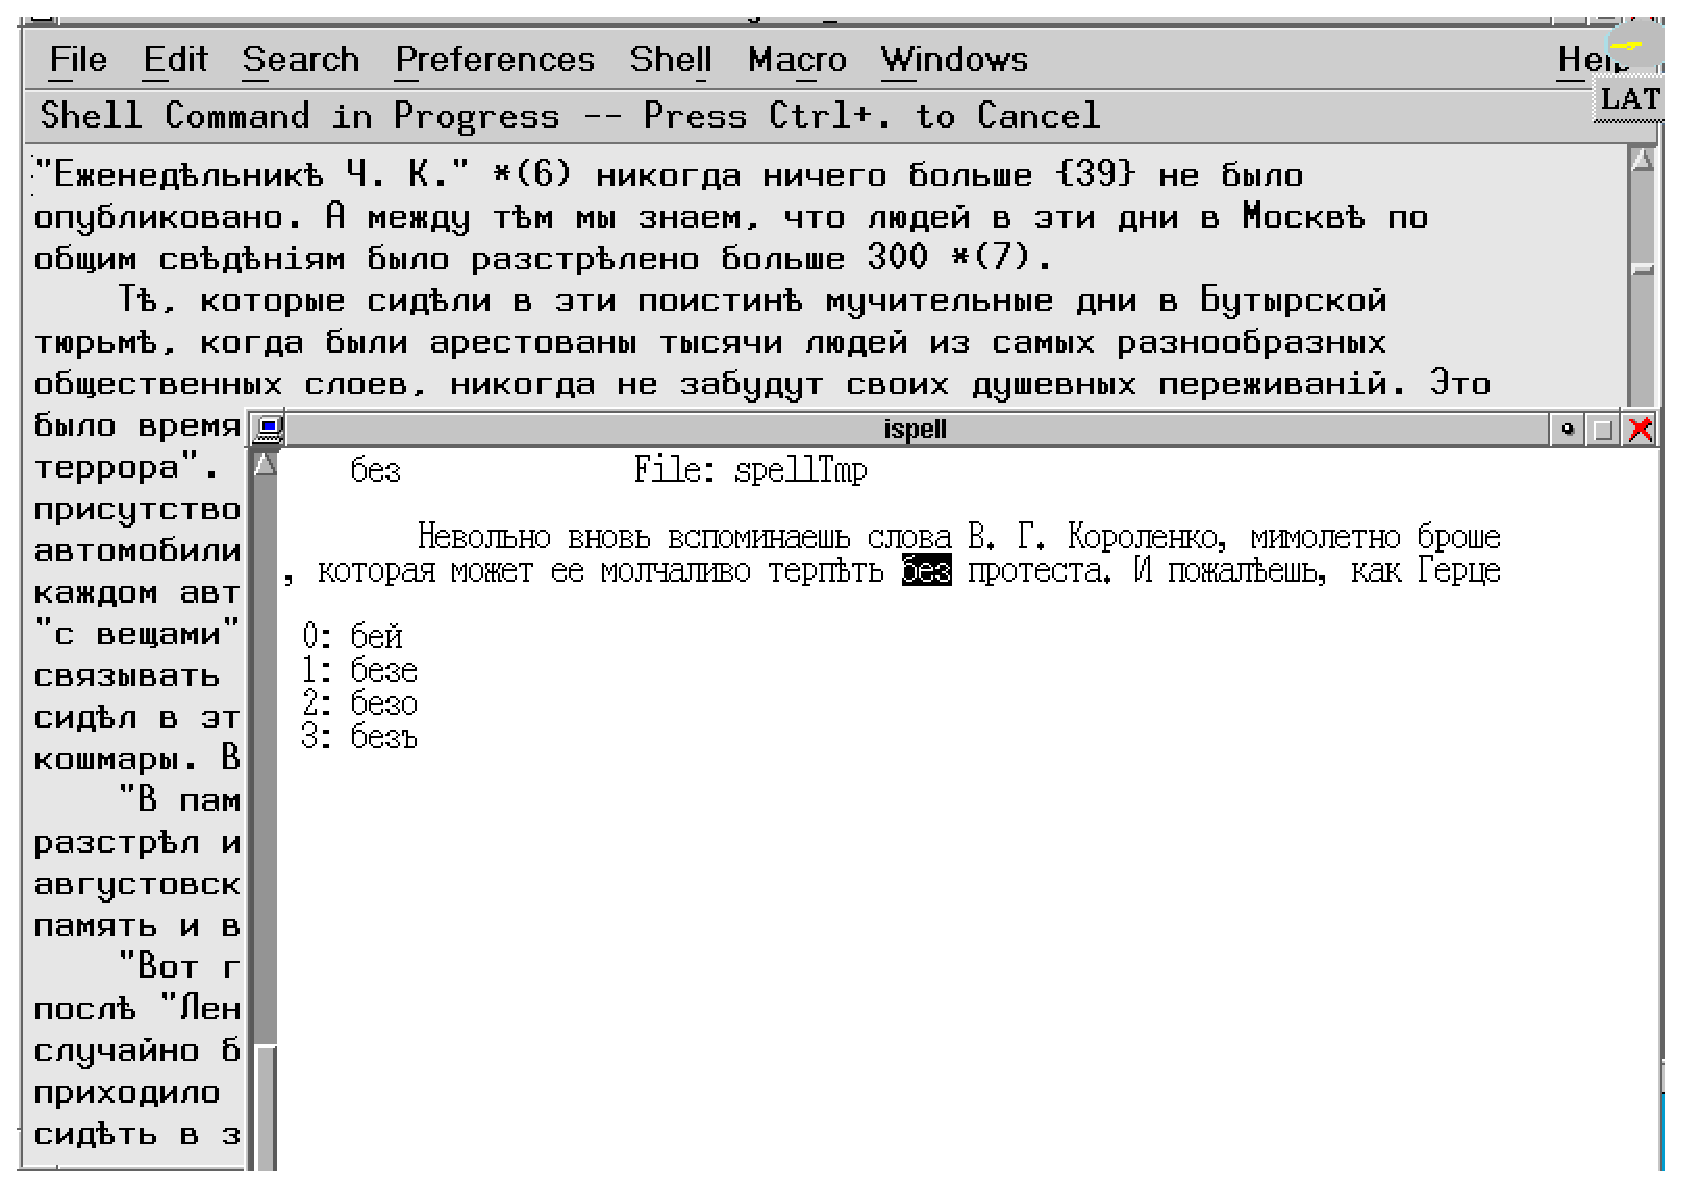
\includegraphics[width=1.2\textwidth]{oldrus-screenshot}
\end{frame}

\begin{frame}{Main linguistic challenge: recover lost information}


To convert texts to the old Russian orthography, we:
\begin{itemize}
\item disambiguate word pairs that became homographs...

\selectlanguage{russian}%
\begin{itemize}
\item самого - самаго, синее - синѣе, оселъ - осѣлъ
\end{itemize}
\selectlanguage{english}%
\item ...and also some homophones that became homonyms

\selectlanguage{russian}%
\begin{itemize}
\item есть - ѣсть, нежить - нѣжить, некогда - нѣкогда
\end{itemize}
\selectlanguage{english}%
\item restore traditional word endings: requires parsing the grammar

\selectlanguage{russian}%
\begin{itemize}
\item {*}они, туманные звезды\foreignlanguage{english}{ $\rightarrow$ }он\textbf{ѣ},
туманны\textbf{я} зв\textbf{ѣ}зды
\end{itemize}
\selectlanguage{english}%
\item restore old letters in word stems, prefixes, and suffixes

\selectlanguage{russian}%
\begin{itemize}
\item \textbf{Ѳ}едоръ \foreignlanguage{english}{(\textbf{Th}eodor), }ор\textbf{ѳ}ографія
\foreignlanguage{english}{(or\textbf{th}ography)}, м\textbf{ѵ}ро \foreignlanguage{english}{(m\textbf{y}rrhe)}
\item {*}рассвирепел $\rightarrow$ ра\textbf{з}свир\textbf{ѣ}п\textbf{ѣ}лъ,
{*}нежнейшего \foreignlanguage{english}{$\rightarrow$} н\textbf{ѣ}жн\textbf{ѣ}йш\textbf{а}го
\end{itemize}
\end{itemize}
\end{frame}

\begin{frame}{Disambiguation tasks}



\begin{itemize}
\item identifying parts of speech

\selectlanguage{russian}%
\begin{itemize}
\item {*}синее $\rightarrow$ синее \foreignlanguage{english}{(blue)}, синѣе
\foreignlanguage{english}{(more blue)}
\item {*}тем $\rightarrow$ темъ \foreignlanguage{english}{(of themes)},
тѣмъ \foreignlanguage{english}{(by that)}
\end{itemize}
\selectlanguage{english}%
\item identifying grammatical forms (number, gender, case, tense)

\selectlanguage{russian}%
\begin{itemize}
\item {*}в море $\rightarrow$ въ море \foreignlanguage{english}{(into the
sea)}, въ морѣ \foreignlanguage{english}{(within the sea)}
\item {*}есть $\rightarrow$ есть \foreignlanguage{english}{(it is)}, ѣсть
\foreignlanguage{english}{(to eat)}
\end{itemize}
\selectlanguage{english}%
\item for some words, identifying \textbf{semantic content} is required

\selectlanguage{russian}%
\begin{itemize}
\item {*}мир $\rightarrow$ миръ \foreignlanguage{english}{(peace)}, міръ
\foreignlanguage{english}{(world)}
\item {*}лечу $\rightarrow$ лечу \foreignlanguage{english}{(I fly)}, лѣчу
\foreignlanguage{english}{(I heal)}
\end{itemize}
\selectlanguage{english}%
\item prononciation details (stress, \foreignlanguage{russian}{е/ё}) sometimes
help 
\end{itemize}
\end{frame}

\begin{frame}{Converter for the old Russian orthography}

\begin{itemize}
\item Dictionary-based, with some simple heuristics
\item No full disambiguation, results need proofreading
\end{itemize}

Tyutchev, \emph{Silentium} (1830)\\



\fbox{\begin{minipage}[t]{0.45\columnwidth}%
\selectlanguage{russian}%
Молчи, скрывайся и таи 

И чувства и мечты свои - 

Пускай в душевной глубине 

Встают и заходят оне 

Безмолвно, как звезды в ночи,- 

Любуйся ими - и молчи.\selectlanguage{english}%
%
\end{minipage}}~%
\fbox{\begin{minipage}[t]{0.48\columnwidth}%
\selectlanguage{russian}%
Молчи, скрывайся и таи 

И чувства и мечты свои - 

Пускай в\textbf{ъ} душевной глубин\textbf{ѣ} 

Встают\textbf{ъ} и заходят\textbf{ъ} он\textbf{ѣ} 

Безмолвно, как\textbf{ъ} зв\textbf{ѣ}зды в\textbf{ъ} ночи,- 

Любуйся ими - и молчи. \selectlanguage{english}%
%
\end{minipage}}

\end{frame}

\begin{frame}{Outlook: the future of the old Russian orthography}

\begin{itemize}
\item Custom keyboard layouts will become standard in OSes?
\item Hyphenation dictionaries for \LaTeX{} and other systems?
\item Spelling dictionaries and grammar checking
\item Fully disambiguating converter between new and old orthography
\end{itemize}
\end{frame}

\end{document}
